\documentclass{beamer}
\usetheme{metropolis}

\usepackage[utf8]{inputenc}
\usepackage[normalem]{ulem}
\usepackage{csquotes}

\title{IDU1321. Ettevõtte äriarhitektuur}
\subtitle{Kolmas loeng}
%\date{10.09.2017}
\author{Andres Kütt}
\institute{Cybernetica, arhitekt}


\begin{document}

\begin{frame}
\titlepage
\end{frame}

\begin{frame}[standout]
Küsimusi loetu kohta?
\end{frame}


\begin{frame}[standout]
Küsimusi kodutöö kohta?
\end{frame}

\section{Kultuur, arhitektuur ja strateegia}
\begin{frame}[fragile]
	\begin{center}
		\LARGE{\textbf{Culture eats strategy for breakfast}}
		\\[4cm]
		\small{Peter Drucker (Mark Fieldsi viide 2006)}
	\end{center}
\end{frame}

\begin{frame}[fragile]
	\begin{center}
		\LARGE{\textbf{Everybody's got a plan until they get hit in the mouth}}
		\\[4cm]
		\small{Mike Tyson}
	\end{center}
\end{frame}


\begin{frame}{Seosed}
	\begin{itemize}
		\item Kultuur tuleneb organisatsioonist ja selle juhtidest
		\item Strateegia kujundab organisatsiooni ja selle juhte
		\item Kultuur toetab strateegia ellu viimist
		\item Ettevõtteerhitektuur toetab strateegia ellu viimist
		\item Kultuur määrab arhitektuuri põhijooned
	\end{itemize}
	
	\begin{center}
		\textbf{Mõttemudel:} Arhitektuur on keha ja kultuur on vaim. \\Eesmärgide saavutamine eeldab mõlemat
	\end{center}
\end{frame}

\begin{frame}[fragile]
	\begin{center}
		\LARGE{\textbf{EA on integraalne osa keerulisest seoste võrgustikust}}
		\\[4cm]
		\small{Arhitekti lisaväärtus tuleneb \\võimest efektiivselt muuta seda, mida muuta saab}
	\end{center}
\end{frame}


\section{Organisatsiooni mudel}
\begin{frame}[fragile]
	\begin{center}
		\LARGE{\textbf{Kõik mudelid on valed, \\mõned mudelid on kasulikud}}
		\\[4cm]
		\small{Iga mudel on definitsiooni järgi lihtsustus lõputult keerulisest maailmast.\\Kuidas mu mudel kasulik on ja kellele?}
	\end{center}
\end{frame}

\begin{frame}[fragile]
	\begin{center}
		\LARGE{\textbf{Organisatsioone saab vaadelda kui süsteeme}}
		\\[4cm]
		\small{Milline on organisatsiooni arhitektuur?}
	\end{center}
\end{frame}

\begin{frame}[fragile]
	\frametitle{Kaks eri vaadet süsteemidele}

	\begin{center}
	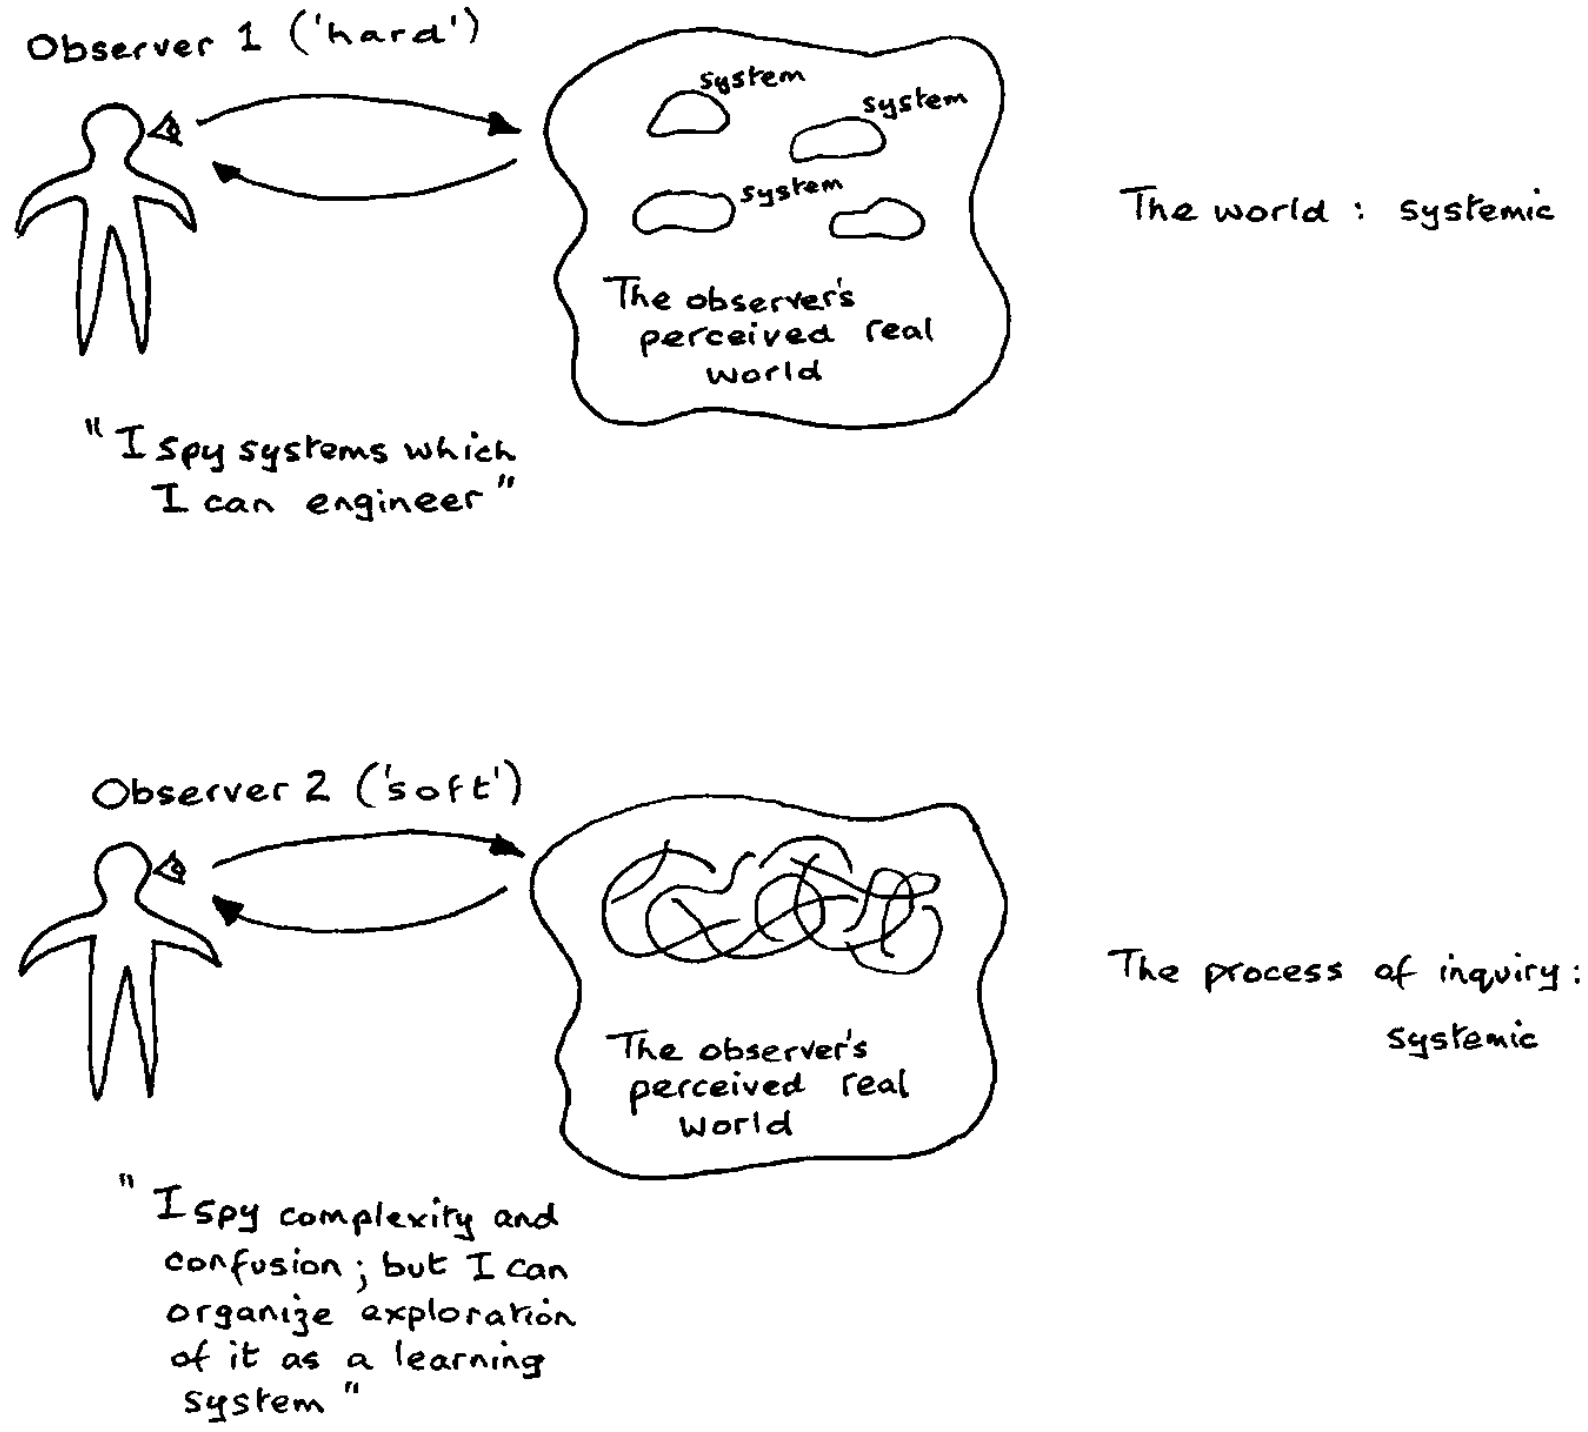
\includegraphics[width=.7\textwidth]{checkland.png}
	
	\cite{checkland2000soft}
	\end{center}
\end{frame}
\begin{frame}
	\frametitle{Kontseptsioon}
		Kuidas organisatsioonist \textbf{mõelda}?
			\begin{itemize}
				\item Strateegia
				\begin{itemize}
					\item Kõige laiemas, organisatsiooni liikmete peas asuvas, tähenduses
					\item Mida vastab keskmine töötaja, kui strateegia kohta küsida?
				\end{itemize}
				\item Organisatsiooni kultuur
				\begin{itemize}
					\item Kogum jagatud uskumusi ja väärtusi
					\item ``Kuidas meil asju aetakse``
				\end{itemize}
				\item Juriidiline struktuur
				\begin{itemize}
					\item Kuidas on organisatsioon kontektsti suhtes defineeritud?
					\item Kas mõtleme kasumile, riigi eesmärkide täitmisele või kogukonna teenimisele?
					\item Väga laias plaanis määrab juriidika, millised on organisatsiooni ja seega ka mõttemudeli piirid
				\end{itemize}				
			\end{itemize}
\end{frame}


\begin{frame}
	\frametitle{Funktsioon}
		Mida organisatsioon \textbf{teeb}?
			\begin{itemize}
				\item Loob omanikule väärtust
				\begin{itemize}
					\item Aga mis on väärtus?
					\item Väga abstraktne ja suhteliselt kasutu formuleering
				\end{itemize}
				\item Järgmine tase on detailne
				\begin{itemize}
					\item Organisatsioonidel on erinevad väärtusprotsessid
					\item Ja üldistust on raske välja tuua
					\item Funktsioonide modelleerimine on keeruline teadus (emergents!)
				\end{itemize}
				\item Mis meid tegelikult huvitab?
				\begin{itemize}
					\item et funktsioon oleks määratletav
					\item et tal oleks mingi sisemine struktuur
				\end{itemize}

			\end{itemize}
\end{frame}

\begin{frame}
	\frametitle{Vorm}
		Millest \textbf{koosneb} organisatsioon?
			\begin{itemize}
				\item Orgvara (ingl. \emph{peopleware})
				\begin{itemize}
					\item Asjad, mida saab juhtida
					\item Üksused, protsessid jne.
					\item Juhtimisteaduse domeen
				\end{itemize}
				\item Tarkvara
				\begin{itemize}
					\item Asjad, mis käivad riistvara sees
					\item Loodud ja COTS tarkvara. Aga ka ruuteri \emph{firmware}
					\item Arvutiteaduse domeen
				\end{itemize}
				\item Riistvara
				\begin{itemize}
					\item Asjad, mille sees käivad kaks eelmist
					\item Serverid, kaablid, külmad toad aga ka kontoripind
					\item Opside (ja kontoriassistendi) domeen
				\end{itemize}
			\end{itemize}
\end{frame}



\begin{frame}[fragile]
	\frametitle{Organisatsiooni arhitektuur}

	\begin{center}
	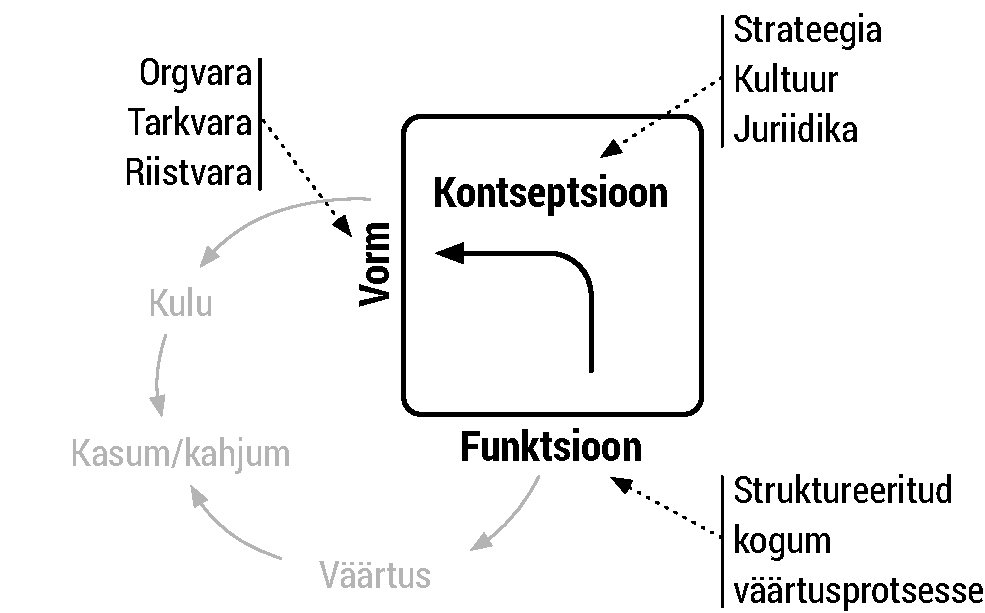
\includegraphics[width=\textwidth]{orgstruktuur.pdf}
	\end{center}
\end{frame}

\begin{frame}[fragile]
	\frametitle{Organisatsiooni arhitektuur}

	\begin{center}
	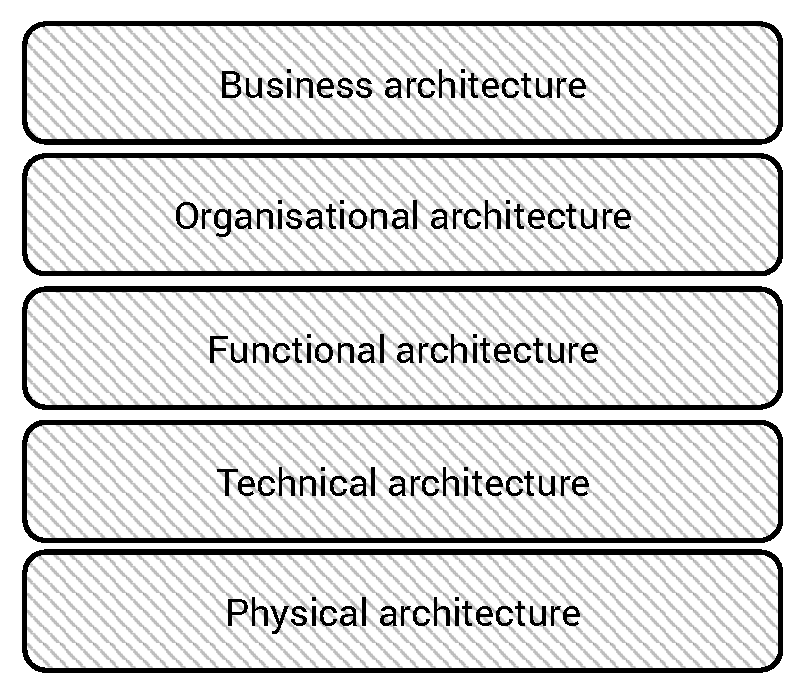
\includegraphics[width=.7\textwidth]{orgmodel.pdf}
	\end{center}
\end{frame}


\section{Harjutus}

\begin{frame}{Lahkame EMTAt}
Ettevõttearhitekti positsioonilt otsime vastust küsimustele:
\begin{itemize}
	\item Mida EMTA teeb?
		\begin{itemize}
			\item Mis väärtust pakutakse ja kellele?
		\end{itemize}
	\item Kuidas EMTAst mõelda?
	\begin{itemize}
		\item Strateegia, juriidika ja kultuur
	\end{itemize}
	\item Millest EMTA koosneb?
	\begin{itemize}
		\item Organisatsioon, tarkvara, füüsiline taristu
	\end{itemize}
\end{itemize}
\end{frame}


\begin{frame}{Harjutuse kokkuvõte}
	\begin{itemize}
		\item Pange tähele, kuidas küsimuste vastused üksteisest sõltuvad. Miks?
		\item Kas sedalaadi pilti on üldse võimalik väljastpoolt organisatsiooni joonistada?
	\end{itemize}
\end{frame}

\begin{frame}[fragile]
	\frametitle{Organisatsiooni arhitektuur}

	\begin{center}
	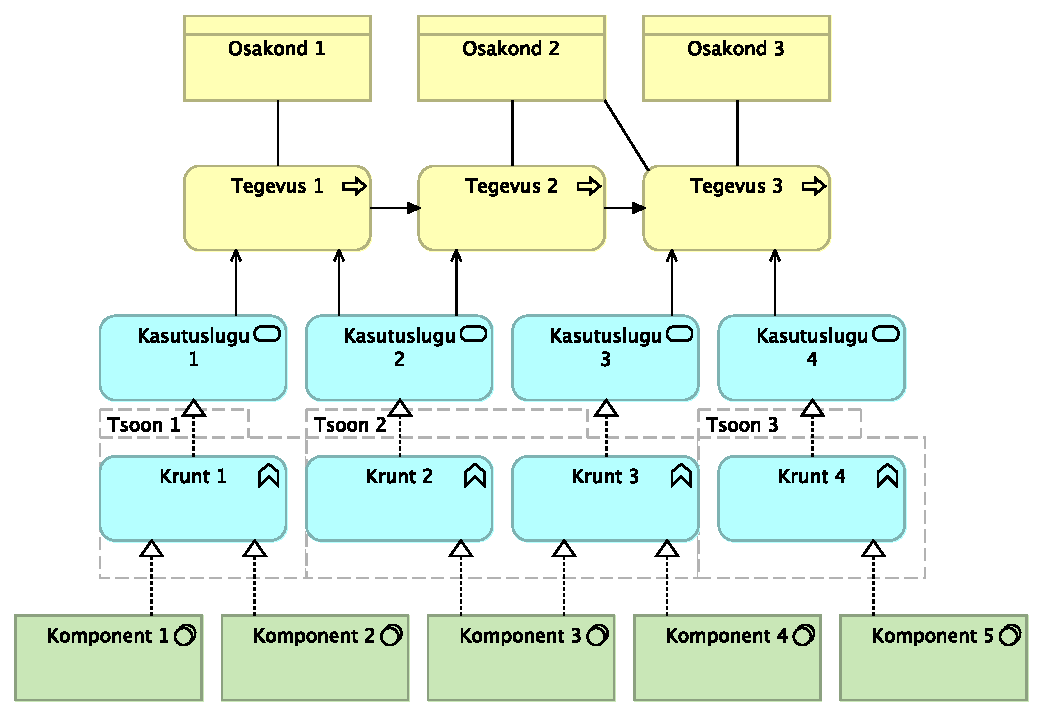
\includegraphics[width=.9\textwidth]{kihid.pdf}
	\end{center}
\end{frame}


\begin{frame}{Kordame}
	\begin{itemize}
		\item Organisatsiooni eri aspektid on üksteisega tihedalt seotud
		\item Keha ja vaim
		\item Organisatsiooni vorm, funktsoon ja kontseptsioon
	\end{itemize}
\end{frame}

\begin{frame}{Järgmine kord}
\begin{itemize}
	\item Äriprotsess ja selle modelleerimine
	\item Kasutuslood ja kasutajalood
	\end{itemize}
\end{frame}

\begin{frame}{Bibliography}
	\bibliographystyle{plainnat}
	\bibliography{idu1321}
\end{frame}

\begin{frame}[standout]
Küsimusi?
\end{frame}

\end{document}
